\documentclass[pdftex,12pt,a4paper]{report}
\usepackage[portuguese,english]{babel}
\usepackage[T1]{fontenc} 
\usepackage[utf8]{inputenc}
\usepackage[pdftex]{graphicx}
\usepackage{minitoc}
\usepackage{hyperref}
\usepackage{indentfirst}
\usepackage[compact]{titlesec}
\usepackage{fancyhdr}
\usepackage{caption}
\usepackage{pgfplots}
\usepackage{pgfplotstable}
\usepackage{fixltx2e}
\usepackage{mathtools}
\usepackage{fancyhdr}
\usepackage{listings}
\usepackage{color}
\usepackage{sverb}

\lstset{language=SQL,%
    %basicstyle=\color{red},
    breaklines=true,%
    keywordstyle=\color{blue},%
    identifierstyle=\color{black},%
    stringstyle=\color{RedViolet},
    commentstyle=\color{mygreen},%
    showstringspaces=false,%without this there will be a symbol in the places where there is a space
    numbers=left,%
    numberstyle={\tiny \color{black}},% size of the numbers
    numbersep=9pt, % this defines how far the numbers are from the text
    emph=[1]{for,end,break},emphstyle=[1]\color{red}, %some words to emphasise
    %emph=[2]{word1,word2}, emphstyle=[2]{style},  
}

\definecolor{Black}{rgb}{0.0, 0.0, 0.0}
\definecolor{Blue}{rgb}{0.0, 0.0, 1.0}
\definecolor{DarkGreen}{rgb}{0.0, 0.42, 0.24}
\definecolor{Red}{rgb}{0.89, 0.0, 0.13}

\lstset{
  breaklines=true,                                     % line wrapping on
  language=SQL,
  frame=ltrb,
  framesep=5pt,
  basicstyle=\normalsize,
  keywordstyle=\ttfamily\color{Blue},
  identifierstyle=\ttfamily\color{Black}\bfseries,
  commentstyle=\color{DarkGreen},
  stringstyle=\ttfamily\color{Red},
  showstringspaces=ture
}

\pagestyle{fancy}
\renewcommand*\thesection{\thechapter\arabic{section}}
\newcommand{\HRule}{\rule{\linewidth}{0.5mm}}


\begin{document}

\begin{figure}[h]
\center

\includegraphics[height=1.5cm]{imagens/logo}
\end{figure}

\begin{center}

\textsc{\large University of Aveiro \\[1cm]\large electronics, telecommunications and computing department}\\[1cm]

\textsc{\large Security \\[1cm]}

\HRule \\[0.5cm]
{ \huge \bfseries Secure Messaging Repository System}\\[0.4cm]
{ \large \bfseries Final project}\\[0.4cm]
\HRule \\[1cm]

\textsc{\small{8240 - INTEGRATED MASTER IN COMPUTER ENGINEERING AND TELEMATICS}}\\[1cm]

\end{center}

\begin{minipage}{0.4\textwidth}

\begin{flushleft} \large
\href{mailto:cristiana.carvalho@ua.pt}{Cristiana da Silva Carvalho }
 \small{\\NMec: 77682 | P1}
\end{flushleft}
\end{minipage}
\begin{minipage}{0.4\textwidth}

\begin{flushright} \large
\href{mailto:danielasimoes@ua.pt}{Daniela Pereira Simões}
\small{\\NMec: 76771 | P1}
\end{flushright}
\end{minipage}\\[1cm]

{\large Teachers: João Paulo Barraca, André Zúquete   }\\[0.5cm]

\vfill

{\large 2017-2018}

 %Titulo do Relatorio
\renewcommand{\headrulewidth}{0pt}

%Cabeçalhos de rodapé
\fancyhead{}
\fancyfoot{}
\rfoot{\thepage}

%Renomear Comandos
\renewcommand*\contentsname{Conteúdos}
\renewcommand*\figurename{Figura}
\renewcommand*\tablename{Tabela}

%Conteúdos, dar paragrafo
\tableofcontents

%Headers
\renewcommand{\thechapter}{}

\clearpage

\section{Introduction}

This project is called the "Secure Messaging Respository System" and aims to develop a system that allows the exchange of messages between users in an asynchronous and secure way. Knowing that all messages will pass through a server (central untrustworthy repository), the system is required to guarantee confidentiality, integrity and authentication of the messages; confirmation of message delivery and preservation of identity. This report is intended to reflect all the decisions taken, as well as the necessary justifications.

\newpage
\section{Requirements}

As previously referenced, the system requires:

\begin{itemize}
\item \textbf{Confidentiality, integrity and authentication of messages}: a message can not be read, modified or injected by a third party.
\item \textbf{Message delivery confirmation}: the readers of the messages must prove that they have read the message.
\item \textbf{Preserving user identity}:a user has a Portuguese Citizen Card attached.
\end{itemize}

\newpage
\section{Server and Client Security Process}

\subsection{Algorithms}

Before starting the implementation, it was needed to decide which algorithms to use; we decided to use hybrid ciphers in most cases, in this way we'll have the speed of the symmetric ciphers but still using the advantages of asymmetric ciphers.

To fill the place of symmetric ciphers we chose AES with CTR mode.
We decided to use AES because it allows large keys (maximum 256) and it's a very strong \footnote{https://blog.agilebits.com/2013/03/09/guess-why-were-moving-to-256-bit-aes-keys/}\footnote{https://wei2912.github.io/posts/crypto/why-aes-is-secure.html} cipher, and with the mode CTR because in this mode we'll have homogeneous access with pre-processing but, plus this, we'll have parallel processing, which makes encryption and decryption faster. Regardless of whether or not it is used in most messages, we don't know the size of the message we'll need to encrypt, so having a fast algorithm which allows parallel processing seems a good choice. 


\begin{figure}[!htb]
\center
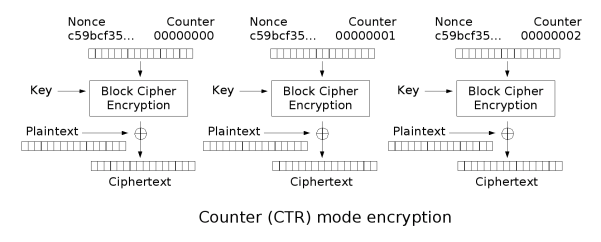
\includegraphics[height=5cm]{imagens/Ctr_encryption.png}
\end{figure}

\begin{figure}[!htb]
\center
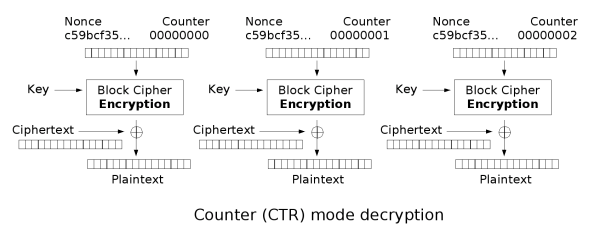
\includegraphics[height=5cm]{imagens/Ctr_decryption.png}
\end{figure}

To fill the place of asymmetric cipher we chose RSA. Despite knowing its disadvantages as being slow to encrypt large data and others, we already use symmetric ciphers to dissolve these problems. And as strong advantages, RSA is a secure algorithm which use complex mathematics and because of this it is considered hard to crack.


\subsection{Session Key}

In order to establish a secure connection with the server, the client generates a initial session key and makes a derivation of that session key per command/response to avoid pattern recognition.

For this effect, Diffie-Helman was considered. This algorithm is a way to exchange keys through a public channel, between two peers to agree on a shared secret. The major advantage of this algorithm is that two peers may have no knowledge about each other and yet can agree on a useful shared secret to establish a secure channel.

It is assumed that a public channel isn't a secure channel, and because of that assumption, it was needed extra implementations that are explained in the next figure.

\newpage

\begin{figure}[h!]
\center
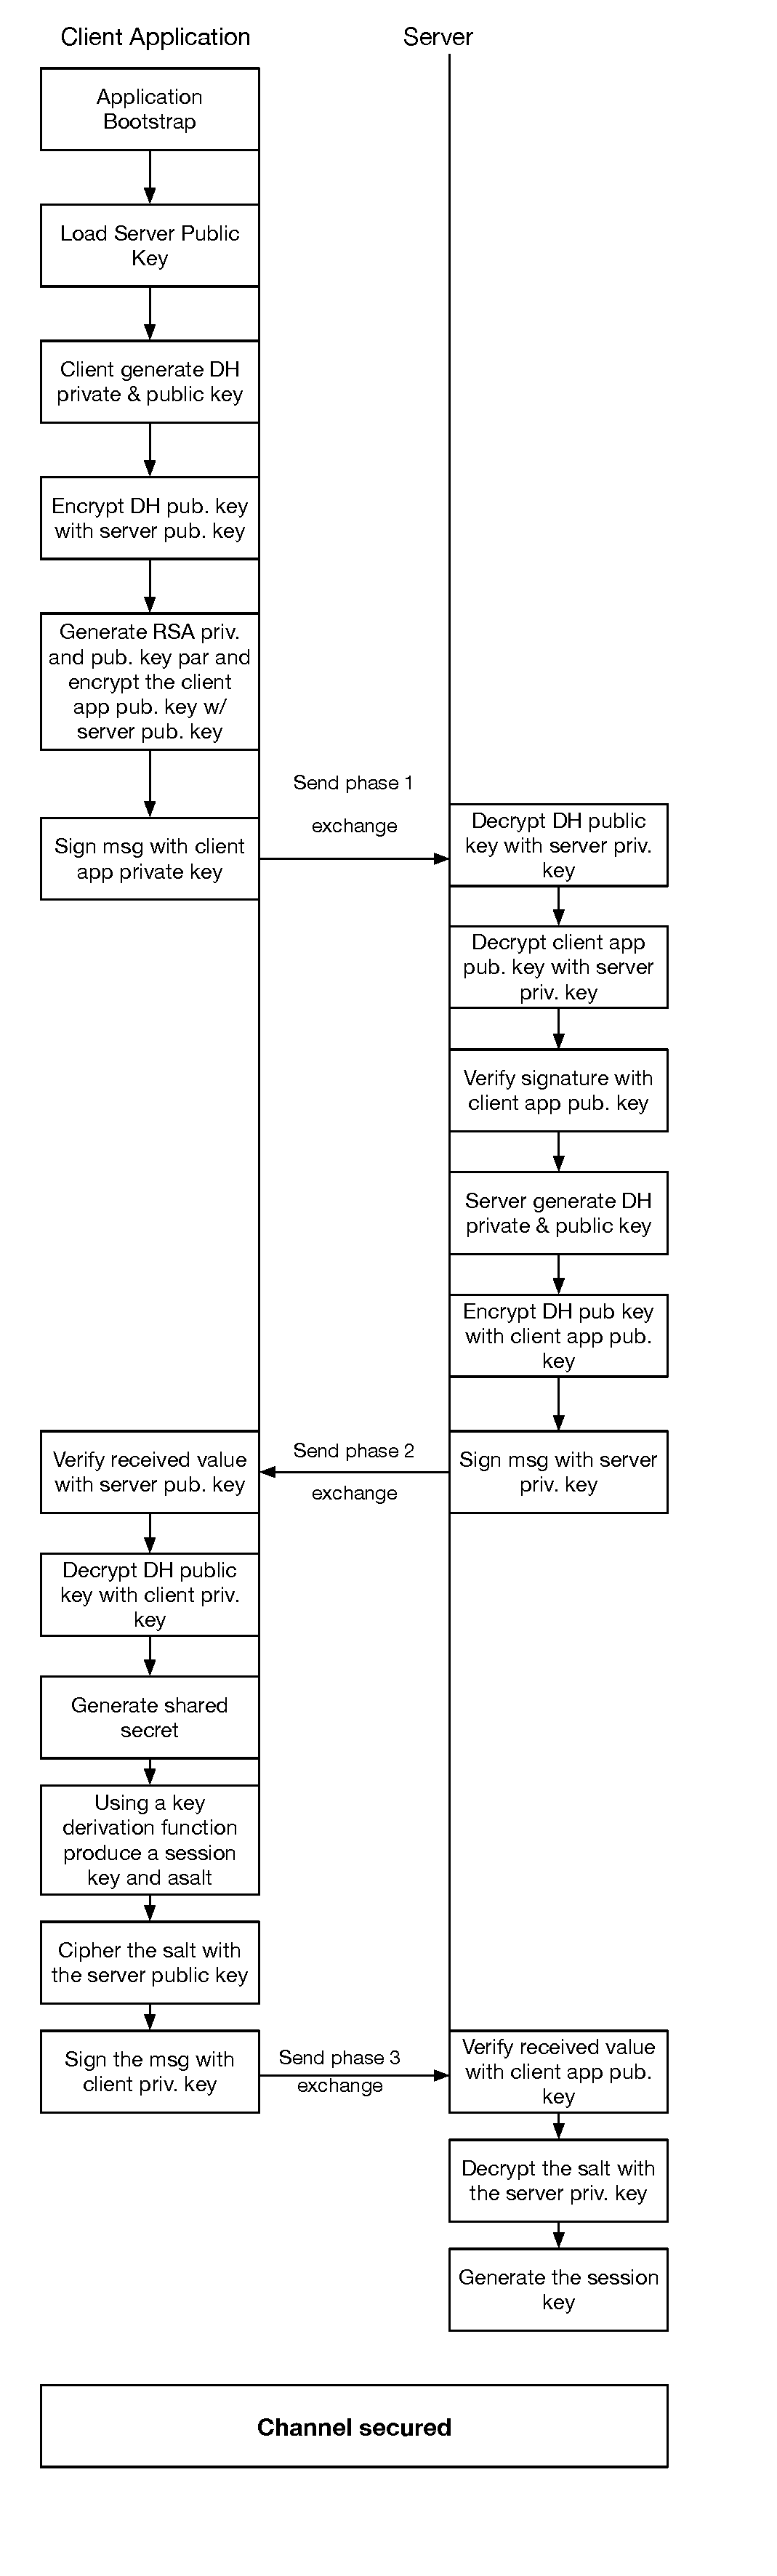
\includegraphics[height=18cm]{imagens/client_app_bootstrap.pdf}
\caption{Session key negotiation.}
\end{figure}

First the client application loads the server public key that is distributed into the client application (it must be verified if the public key of the server is still the same; if not, it must be updated).

After that, the client app generate DH values (private and public) to exchange with the server in order to get the shared secret.

\begin{itemize}
    \item Phase 1 [CLIENT]: Send generated DH public key to the server and the app client RSA public key. Everything is signed and ciphered with a hybrid cipher (using AES and RSA).
    
\textbf{Hybrid Cipher used:}
\begin{lstlisting}[language=Python]
def hybrid_cipher(self, obj, public_key, ks=os.urandom(32), cipher_key=True):
    iv, ciphered_obj = self.sym_cipher(obj, ks)
    iv_encrypted = self.asym_cipher(public_key, iv)

if cipher_key:
    key_encrypted = self.asym_cipher(public_key, ks)
    pickle_dumps = pickle.dumps([{
    "obj": base64.b64encode(ciphered_obj).decode(),
    "iv": base64.b64encode(iv_encrypted).decode(), 
    "key": base64.b64encode(key_encrypted).decode()}, os.urandom(RANDOM_ENTROPY_GENERATOR_SIZE])
    return base64.b64encode(pickle_dumps)
else:
    pickle_dumps = pickle.dumps([{
    "obj": base64.b64encode(ciphered_obj).decode(),
    "iv": base64.b64encode(iv_encrypted).decode()},os.urandom(RANDOM_ENTROPY_GENERATOR_SIZE)])
    return base64.b64encode(pickle_dumps)
\end{lstlisting}

    \item Phase 2 [SERVER]: the server generates the private and public DH pair. Then using the server private key, the server decipher the received encrypted value (DH public key from client). Using again the server private key, the server deciphers the client public key and loads it into memory.
    Then, using the client public key, validates the signature made for the DH public value and public key received.
    Using the received client public key, the server will use a hybrid cipher (AES and RSA) to encrypt the generated DH public key. After the cipher, the server will sign everything with the server private key.

    \item Phase 3 [CLIENT]: using the stored server public key, the client will validate the signature received. After
    that, using the client private key, the client will decipher the DH public value received from the server. Afterwards, using the DH public value, the client will generate the DH shared secret. The generated shared secret will be a "master key" where will be applied a function from the library PBKDF2HMAC, that will derivate other keys from the master key. To derivation was chosen to have 100 000 iterations. The salt is a random value and so, it will be ciphered and sent to the server.
    The session key has been generated.

\begin{lstlisting}[language=Python]
def key_derivation(self, masterkey, salt=os.urandom(32), iterations=100000):
    kdf = PBKDF2HMAC(
        algorithm=hashes.SHA512(),
        length=32,
        salt=salt,
        iterations=iterations,
        backend=default_backend()
    )
    
    return kdf.derive(masterkey), salt
\end{lstlisting}

    \item Phase 4 [SERVER]: Using the client public key it will be verified the signature of the received value. Using the server private key and a hybrid cipher, the PBKDF2 salt will be deciphered. Using the key derivation function the session key will be obtained in the server.
    Finally, there is a secure channel between the server and the client.

\end{itemize}

To avoid Man In The Middle Attacks, the exchanged values in the session key negotiation were ciphered and signed, in this way, it's possible to guarantee the authenticity, confidentiality and integrity.

It was decided to not use HMAC or other type, considering that is already used digital signatures which provide everything HMAC would.

Some steps described above don't have to be executed necessarily in the written sequence.

\subsection{Server commands/response cipher}

In the first moment we thought to use two modes: one for short messages and other for long messages; but with CTR we think we can apply to both type of messages considering its speed  \footnote{http://www.cs.wustl.edu/~jain/cse567-06/ftp/encryption_perf/index.html}, and reliability.

The key used will be a derivation of the Session Key (Master Key). For the CTR mode we decided to generate a random IV (to make attacks difficult) and exchange it with the server. For that, we need to cipher the IV (16 bytes, to avoid repetitions) with a asymmetric cipher.

\subsubsection{Client request cipher}

When a command from the client is built, the client encapsulates it with a secure layer. The secure layer is a process that:

\begin{itemize}
    \item {
        Produces a nounce with the command content and concatenates with a 32 bytes random hexadecimal number to add some entropy.
    } 
    \item {
        Using a key derivation function, the initial session key (as master key) and the number of requests made to the server (only the client and the server know how many requests were made since the channel has been established) it will be generated a key (and a salt) to be used in the cipher of the message. The IV (16 bytes) needed for the symmetric cipher will be generated and saved.
    }
    \item{
        The key used above and the number of iterations are the only elements that the server knows. To pass the missing elements to the server it will be made a dictionary with the salt, nounce and iv value. Then, that dictionary will be ciphered (using hybrid cipher) with the server public key.
    }
    \item{
        The message content will be ciphered with a symmetric cipher (above mentioned) using the previous result key and IV.
    }
    \item{
        All the composed message will be signed with the client app private key. And the server will be capable of verify the signature because in the first exchange of messages, the public key of the client app is sent.
    }
\end{itemize}


\begin{lstlisting}[language=Python]
    def secure_layer_crypt(self, msg: bytes):
        nounce = sha256(json.dumps(msg).encode() + os.urandom(32)).hexdigest().encode()
        key, salt = self.key_derivation(self.session_key, iterations=self.request_to_server)
        iv = os.urandom(16)

        self.warrant_nounces[nounce] = {"iterations": self.request_to_server, "salt": salt}

        sec_data = pickle.dumps({
            "salt": salt,
            "nounce": nounce,
            "iv": iv
        })

        sec_data_ciphered = self.hybrid_cipher(sec_data, self.server_pub_key)

        iv, ciphered_obj = self.sym_cipher(msg, key, iv=iv)

        return_message = {
            "data": base64.b64encode(ciphered_obj).decode(),
            "sec_data": base64.b64encode(sec_data_ciphered).decode()
        }

        return_message["signature"] = base64.b64encode(self.asym_sign(self.client_app_keys[0], json.dumps(return_message).encode())).decode()

        self.request_to_server += 1

        pickle_dumps = pickle.dumps(return_message)

        return base64.b64encode(pickle_dumps)
\end{lstlisting}

\subsubsection{Client request decipher}

The server receives the composed message and deciphers the secure layer with the following process:

\begin{itemize}
    \item {
        The message signature is verified with the previous received client public key.
    } 
    \item {
        Using the server private key, the missing elements to decipher the message will be decipher using a hybrid cipher.
    }
    \item{
        Using the received salt from the server, knowing the number of requests received by the client, the server with the session key (master key) will make the derivation to a new session key.
    }
    \item{
        Using that key and IV, the server will decipher the message content.
    }
    \item{
        The used salt, nounce and iterations are saved in order to be part of the genuine warrant and compose the response message. 
    }
\end{itemize}

\begin{lstlisting}[language=Python]
def secure_layer_decrypt(self, msg: bytes):
    msg = pickle.loads(base64.b64decode(msg))

    data = msg["data"].encode()
    sec_data = base64.b64decode(msg["sec_data"])

    signature = base64.b64decode(msg["signature"].encode())
    del msg["signature"]

    # verify signature
    self.asym_validate_sign(json.dumps(msg).encode(), signature, self.client_public_key)

    iterations = self.requests_received
    self.requests_received += 1

    # decipher the sec_data
    sec_data = pickle.loads(self.hybrid_decipher(sec_data, self.server_priv_key))

    salt = sec_data["salt"]
    nounce = sec_data["nounce"]
    iv = sec_data["iv"]

    key, salt = self.key_derivation(self.session_key, iterations=iterations, salt=salt)

    raw_msg = self.sym_decipher(base64.b64decode(data), key, iv)

    data = {"nounce": nounce,
            "salt": salt,
            "iterations": iterations}

    return raw_msg, data
\end{lstlisting}

\subsubsection{Server response cipher}

The response that the server made for a given request is ciphered using the same values of the request. In the sec\_data received dictionary there are the salt and the iterations used to make the derivation from the master key.

The nounce received is sent back to the client ciphered using a hybrid cipher (with the client public key).

After that, all the message is signed with the server private key, including the nounce, proving that the client made that response for the given request (identified by the nounce).

\begin{lstlisting}[language=Python]
def secure_layer_encrypt(self, msg: bytes, sec_data: dict):
   key, salt = self.key_derivation(masterkey=self.session_key, salt=sec_data["salt"], iterations=sec_data["iterations"])

    ciphered_msg = self.hybrid_cipher(msg, self.client_public_key,
                                      ks=key,
                                      cipher_key=False)

    sec_data = pickle.dumps({
        "nounce": sec_data["nounce"]
    })

    # sec_data ciphered
    sec_data_ciphered = self.hybrid_cipher(sec_data, self.client_public_key)

    return_message = {
        "data": ciphered_msg.decode(),
        "sec_data": base64.b64encode(sec_data_ciphered).decode()
    }

    return_message["signature"] = base64.b64encode(self.asym_sign(self.server_priv_key, json.dumps(return_message).encode())).decode()

    # dump the return message
    pickle_dumps = pickle.dumps(return_message)

    return base64.b64encode(pickle_dumps)
\end{lstlisting}

\subsection{Genuineness server reply warrant}

When the client is building the request it appends extra information to the message. It appends a unique hash built with a NOUNCE (made of an hash of the message concatenated with a 32 byte hexadecimal random number). The hash is appended to the secdata, such as the salt and the IV generated. These values are also stored in the client side to make the verification later.

The server will keep the received values, and append the exactly same NOUNCE to the response, and sign.
Now, in the client side, the client will verify the signature and decipher everything. Then, the client have to make the NOUNCE verification. If the NOUNCE is equal to the one that itself sent, then we assume the response is the one which matches the sent request, else an error is shown.

In the end, the NOUNCE is deleted from the client, to avoid the remote possibility of equal NOUNCES to different requests.

In this way, we can assume that the response came from the server (because of the signature - non repudiation) and that's confidential (because was ciphered with client public key). And, the most important to this topic, that the response belongs to the sent request, because in the response must exist an unpredictable value that the client validates and guarantees that is equal to the one the client sent or not.


\subsection{Integrity control}

When a client application bootstraps, it generates a private and public key, then when the client negotiates with the server for the first time, it will send a public key to be used in the integrity and authenticity control by the server and it already has the server public key.

When a command is sent, the client application will hash (with SHA-256) the command content and then sign with the private key. When received at the server, it will verify the message with the client public key.

When a response is sent, the server will hash (with SHA-256) the response content and then sign with the server private key. When received at the client app, it will verify the message with the server public key.

\section{User to User cipher}

\subsubsection{Validation of the trust chains}

To be sure that the received certificates are valid, it's needed to verify the trust chain of the Citizen Card Authentication Certificate. Later we'll talk about verifying the trust chain of the Citizen Card Authentication Certificate, and that's how it's done.

First, we needed to download all the chain certificates from the course page. Then we had to load them from DER format into PEM format.
Then, we downloaded from \href{http:/pki.cartaodecidadao.pt}{"Cartão do Cidadão"} the CRLs and load them to verify if the certificate was revoked.

For example, when getting the public information of a user:
\begin{lstlisting}[language=Python]
def get_user_public_details(self, user_id):
    msg = {"type": "user_public_details", "id": user_id}
    self.sck_send(msg)

    peer_public_details = self.sck_receive()["result"]
    signature = peer_public_details["signature"]
    del peer_public_details["signature"]

    chain = []
    for crl in [f for f in os.listdir("utils/crts") if os.path.isfile(os.path.join("utils/crts", f))]:
        chain.append(open(os.path.join("utils/crts", crl), "r").read())

    CitizenCard.validate_chain(chain=chain, pem_certificate=peer_public_details["cc_public_certificate"].encode())

    CitizenCard.verify(json.dumps(peer_public_details).encode(), base64.b64decode(signature.encode()), peer_public_details["cc_public_certificate"].encode())

    return peer_public_details
\end{lstlisting}


\begin{lstlisting}[language=Python]
@staticmethod
def validate_chain(chain, pem_certificate, ssl_ca_root_file="./utils/ca-bundle.txt"):
    trusted_certs_pems = parse_file(ssl_ca_root_file)

    store = crypto.X509Store()

    store.set_flags(crypto.X509StoreFlags.CRL_CHECK)
    store.set_flags(crypto.X509StoreFlags.CRL_CHECK_ALL)

    for pem_crt in trusted_certs_pems:
        store.add_cert(crypto.load_certificate(crypto.FILETYPE_PEM, pem_crt.as_bytes()))

    for pem_crt in chain:
        store.add_cert(crypto.load_certificate(crypto.FILETYPE_PEM, pem_crt))

    certificate = crypto.load_certificate(crypto.FILETYPE_PEM, pem_certificate)

    store_ctx = crypto.X509StoreContext(store, certificate)

    for crl in [f for f in os.listdir("utils/crls") if os.path.isfile(os.path.join("utils/crls", f))]:
        store.add_crl(crypto.load_crl(crypto.FILETYPE_PEM, open(os.path.join("utils/crls", crl), "r").read()))

    store_ctx.verify_certificate()
\end{lstlisting}


\subsection{Register relevant security-related data in the user creation}

When a user is created, it's also created an UUID, generated using his/her own Citizen Card, making a SHA-224 of the Citizen Card Authentication Certificate PEM. This value is stored with the used certificate and a new public key related to the UUID generated. This new public key is needed because Citizen Card private key couldn't decrypt values encrypted by its own public key. These values are signed by the client's Citizen Card private key and stored in the server.

The server before storing all the values, must verify the trust chain of the received certificate and validate the signature.

\subsection{User-User messages cipher}

To guarantee that the sent message is read only by the receiver user it's needed to cipher the message content in order to be stored in the server repository without getting deciphered.

Only the receiver user will have capabilities to decipher the message content. For this effect we store the public key of all registered clients and when an user decides to send a message to another user it will:

\subsubsection{Request the public key of the destination user}

The user who wants to send a message must request to the server some information about the destination user, then the server replies with the Citizen Card Authentication Certificate of destination user, the new public key generated (above explained), the destination user UUID and the signature of all info described by destination user Citizen Card private key. When the user who wants to send a message receives all this data, must verify the signature, and validate the Citizen Card Authentication Certificate trust chain.

\subsubsection{Encrypting the message}

The message will be encrypted with an hybrid cipher already explained above. The message content is encrypted with AES (CTR mode) using a random key (Ks). This Ks is encrypted using the destination user public key, and in this way, the server won't be able to decrypt any information of the stored message. All is signed by the user with its own Citizen Card private key.

\subsubsection{Destination user reads the message}

The destination user asks the server for new messages, and the server replies with the stored new message. The destination client is able to validate the signature of the source user (requesting the public details stored in the server), and decrypt the Ks with its own private key. Once the destination user has the Ks, can decrypt the content message and read it.

\subsubsection{Prevent a user from reading messages from other than their own message box}

The user can read a message from their own message box because the messages in the message box are encrypted with its own public key, in this way, if he/she uses its own private key, they can read the content of the messages. But if they try to decrypt a message from other message box than their own, they won't be able to use their own private key to decrypt the messages, considering that all private keys are safe.

\subsection{Receipts}

\subsubsection{Message send copy}

When a user composes a message, the message sent to the server has a "copy" field. That field is encrypted with the hybrid cipher with the sender public key, guaranteeing that only the sender can read the copied message.

\subsubsection{Destination user reads the message}

When the user reads the message, the user will sign the message content with his/hers Citizen Card private key, proving that he/she actually read the message. Then, using the sender public key, uses a hybrid cipher to encrypt the signed content before, in order to only allow the sender to confirm the signature.

\subsubsection{Check receipts of sent messages}

The sender requests to the server for receipts of a given message (status), and only the sender can read the "message" field of the server response, because it was previously encrypted with its public key.

\subsubsection{Avoiding false receipts}

In order to prevent that user send receipts relatively to messages that she/he didn't read we decide to not use NOUNCEs again, and instead, make the destination user to sign the content of the decrypted message with its own Citizen Card private key, and encrypt with the public key of the sender. This way, the sender will be sure that the destination user opened the message, when he/she validates the signature.

\section{How to run}

This code only works on Python 3.6+.

First, install the requirements present in the folder client and server. 

\$ pip3 install -r requirements.txt

Then run the server with:

\$ python3 server.py

And then run the client:

\$ python3 client.py

\section{Conclusion}

All solutions of the project were based on the achieve knowledge so far.

The present version of the project doesn't contemplate the extras, but we will implement them and deliver the in the "Época de Recurso", trying to achieve the best grade possible.

The project has been very interesting on working on, and we hope we can do better next phase.

\newpage
\section{References}
\begin{itemize}  
\item Slides provided by the discipline.
\item Security in Computer Networks, 4th Edition Augmented, André Zúquete
\end{itemize}


\end{document}